\documentclass[a4paper]{article}
\usepackage{graphicx}
\usepackage{tikz}
\usepackage[
    a4paper,
    margin=0pt
]{geometry}
\usetikzlibrary{matrix,calc}
\input{../commands.tex}
\begin{document}
\cardpage{
    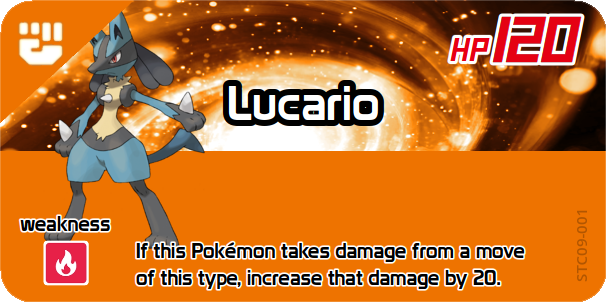
\includegraphics[width=6cm,height=3cm]{../../../../database/cards/characards/STC09-001_lucario}      \&
    
\includegraphics[width=6cm,height=3cm]{../../../../database/cards/wazacards/ST/09-001_lucario/STW09-001.png}\&
    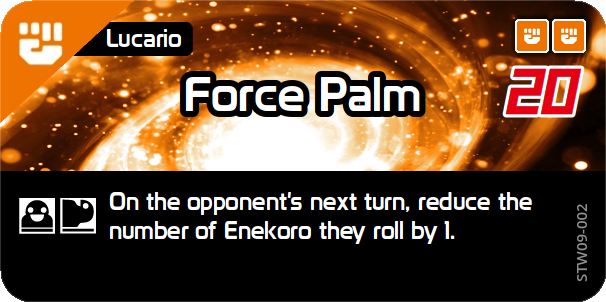
\includegraphics[width=6cm,height=3cm]{../../../../database/cards/wazacards/ST/09-001_lucario/STW09-002.png}\& \\
    
\includegraphics[width=6cm,height=3cm]{../../../../database/cards/wazacards/ST/09-001_lucario/STW09-003.png}\&
    
\includegraphics[width=6cm,height=3cm]{../../../../database/cards/wazacards/ST/09-001_lucario/STW09-004.png}\&
    
\includegraphics[width=6cm,height=3cm]{../../../../database/cards/wazacards/ST/09-001_lucario/STW09-005.png}\& \\
    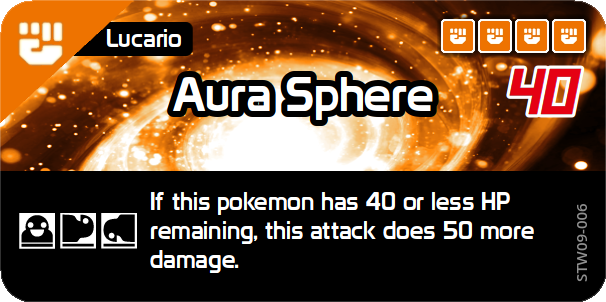
\includegraphics[width=6cm,height=3cm]{../../../../database/cards/wazacards/ST/09-001_lucario/STW09-006.png}\&
    
\includegraphics[width=6cm,height=3cm]{../../../../database/cards/wazacards/ST/09-001_lucario/STW09-007.png}\& \\
}

\end{document}
